
\chapter{Methodology}

This chapter presents the approach used for this research.
 Fig. \ref{phd-methodology} summarizes the steps.

\begin{figure}[h]
\centering
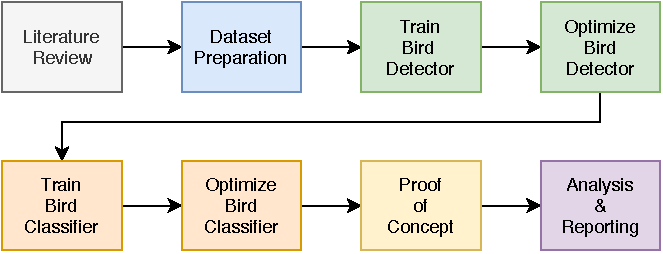
\includegraphics[width=.8\textwidth]{phd-methodology}
\caption{Research methodology.}
\label{phd-methodology}
\end{figure}

\begin{enumerate}
\item To develop 20-species classifier.
\item The number 20 comes from the list of Malaysian Garden birds
\item N shall run 8-bit integer input and parameters
\item Proof on Concept to be run on Raspberry Pi single board computer
\item Raspberry Pi can run acoustic event recognition faster than real time for some large neural networks \citep{Ebbers2018}
\end{enumerate}

 Fig. \ref{cascade-dataflow} summarizes the data flow.


\begin{figure}[H]
\centering
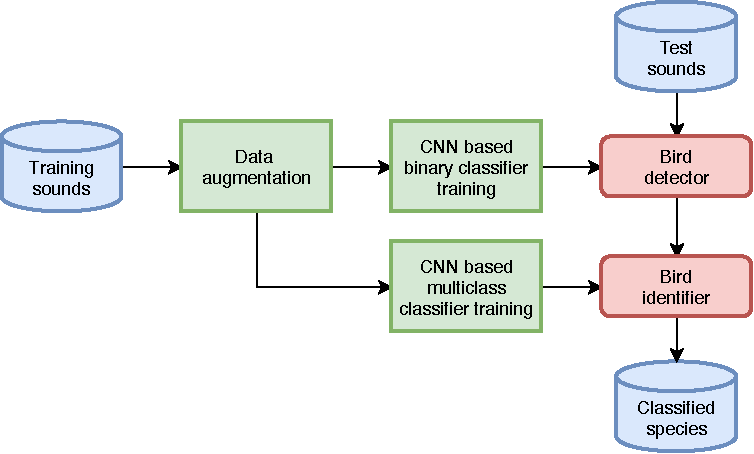
\includegraphics[width=.8\textwidth]{cascade-dataflow}
\caption{Data flow in proposed cascade bird classifier.}
\label{cascade-dataflow}
\end{figure}

\section{Dataset}

 Bird sound dataset not readily usable for deep learning training.
Long sound files to be segmented to 1s clipped, resampled to 8kHz.

\begin{table}[h]
    \centering
    \small
    \caption{Some common bird sound databases.}
	\begin{tabular}{ll}
	\toprule
	\textbf{Dataset} & \textbf{URL} \\
	\midrule
	Xeno-canto & http://xeno-canto.org \\
	Macaulay Library & https://www3.macaulaylibrary.org/browse/taxa/aves \\
	DCASE & http://dcase.community/challenge2018/task-bird-audio-detection \\
	British Birdsong Dataset & https://www.kaggle.com/rtatman/british-birdsong-dataset \\
	LifeCLEF 2018 Bird & https://www.crowdai.org/challenges/lifeclef-2018-bird-monophone \\
	\bottomrule
	\end{tabular}
\end{table}	
	


\section{Bird Detector}


\begin{itemize}
	\item Binary Classifier: Bird/No-bird
	\item Always on: must be simple
	\item When this module detects a possible bird sound, 
			it passes the data to the bird species classifier
	\item Algorithm for this module are based on:
	\begin{itemize}
		\item Voice activity detection for speech recognition
		\item Sound event detection for security
	\end{itemize}
	\item This module must be accurate enough (high TP+FP). FP are taken care by the next module.
\end{itemize}


The bird detector performs the initial detection.
It is as simple as possible as it must run continuously.
The proposed architecture is based on the binarized convolutional neural network (BNN) proposed by \cite{Courbariaux2016}.

	\begin{itemize}
		\item
		The sound detector must listen to continuously streaming audio, ignoring nearly all of it, yet still triggering correctly and instantly.
%		\item
%		On a mobile device, this is particularly challenging when considering that typical mobile devices (e.g. smartphones) have batteries with capacities between 1,000mAh and 2,400mAh
		\item
		Entire system should consume < 1mA to consume < 1\% of the battery per day. \citep{Gruenstein2017}
	\end{itemize}

\begin{figure}
    \centering
    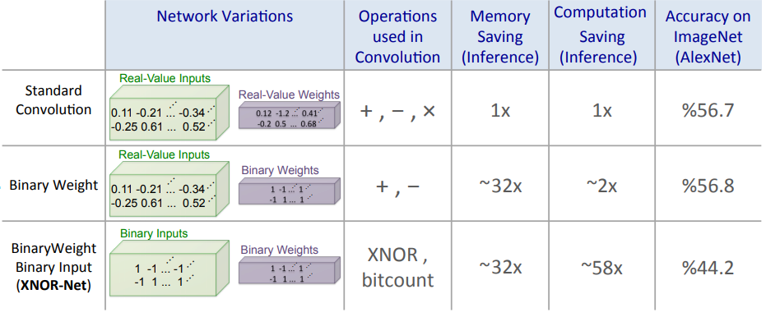
\includegraphics[width=.8\textwidth]{bnn-advantage}
    \caption{Comparison of standard convolution, binary weight/standard input and binary weight/binary input \citep{Rastegari2016}.}
    \label{bnn-advantage}
\end{figure}

\begin{figure}
    \centering
    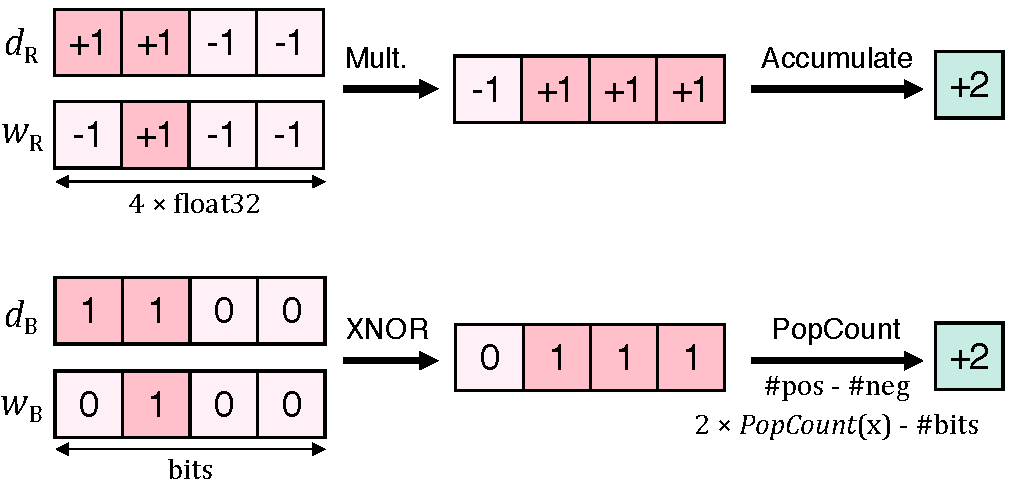
\includegraphics[width=.6\textwidth]{bnn-popcount}
    \caption{Acceleration of binarized neural network by replacing multiply and acummulate operators with XNOR and population count operators, respectively \citep{Rastegari2016}.}
    \label{bnn-popcount}
\end{figure}


\begin{figure}
    \centering
    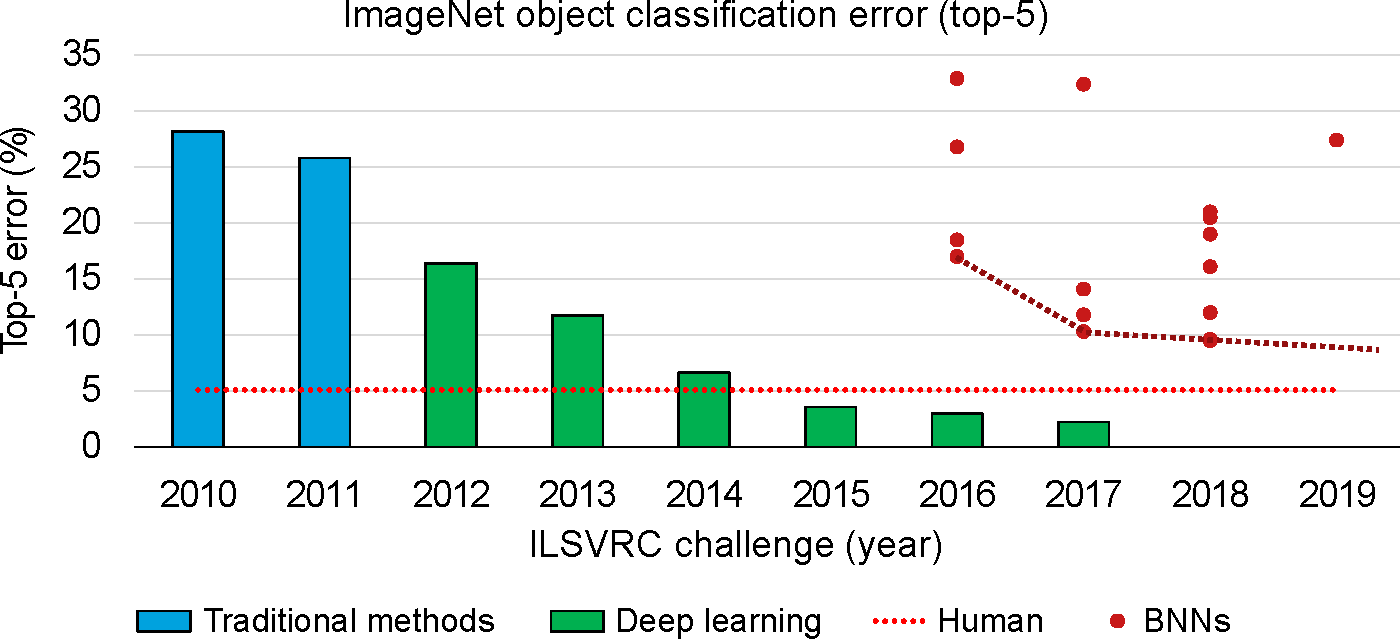
\includegraphics[width=.8\textwidth]{bnn-challenge}
    \caption{BNN still have some catching up to regular CNNs \citep{Rastegari2016}.}
    \label{bnn-challenge}
\end{figure}
\section{Bird Classifier}

 The classifier algorithm has to be lightweight to fit the embedded platform
 Popular CNN does not match the input image square vs elongated
 Use of an existing DNN model as a base, 
			then modified to find the best parameters for bird sound.

\begin{table} 
    \small
    \centering
    \caption{Hand-crafted CNN for bird recognition.}
    \begin{tabular}{lrrrrrrr}%{.15\textwidth}p{.4\textwidth}p{.35\textwidth}}
    \toprule
    \textbf{Reference} & 
    \textbf{DNN } &
    \textbf{layers} &
    \textbf{param.} &
    \textbf{MAC} &
    \textbf{acc.} \\
    \midrule
    \cite{Takahashi2016} & - & 9 & 257M & ? & 92.8 \% \\
    \cite{Grill2017} & bulbul & 8 & ? & ? & ?\\
    \cite{Grill2017} & sparrow & 10 &  ? & ? & ?\\
    \cite{Meyer2017} & custom x 3 & 8 & 233-452 M & 1239-2655 M & 80.3-86.0 \% \\
    \cite{Ruff2019} & custom & 6 & - & - & 63.1-92.5\% \\ %500x129 res, 7 species
    \bottomrule
    \end{tabular}
\end{table}

\subsection{STFT)}

\subsection{Gammatone)}

\subsection{CQT Spectrogram)}

\begin{figure}[H]
\centering
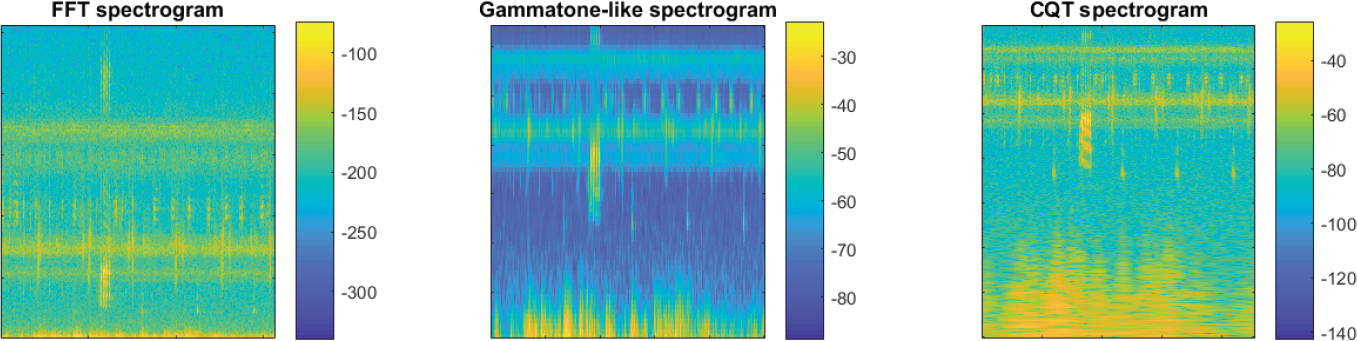
\includegraphics[width=.8\textwidth]{fft-gfcc-cqt}
\caption{STFT, Gammatone and CQT spectrograms \citep{Xie2017}.}
\end{figure}

\FloatBarrier

\subsection{Spectral Image Features (SIF)}

\begin{figure}[h]
\centering
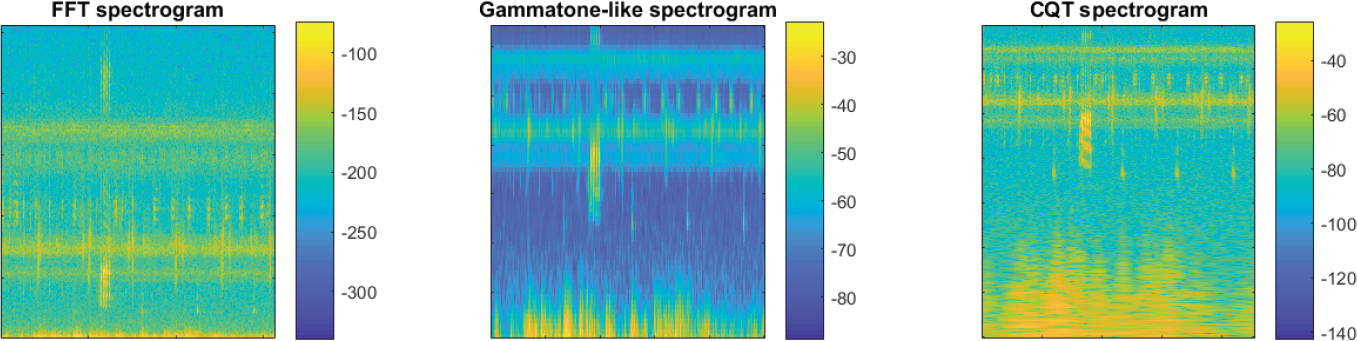
\includegraphics[width=.8\textwidth]{fft-gfcc-cqt}
\caption{STFT, Gammatone and CQT spectrograms \citep{Xie2017}.}
\end{figure}


Detect the bird vocalizations using \cite{Fodor2013}, \cite{Lasseck2015} and \cite{Potamitis2015}.



\section{Training process}

The downloaded sound files will be used to train the networks under consideration.

\section{Evaluation}


To evaluate the performance of each model, we employ the following metrics:

\subsubsection{Precision}

This metric is defined as the proportion of true positives that are correctly identified by the detector. 
This metric is calculated by taking into account the True Positives (TP) and False Negatives (FN):

\[
\mathrm{Precision} = P = \frac{TP}{TP + FN}
\]

\subsubsection{Accuracy}

\[
\mathrm{Accuracy} = \frac{TP+TN}{\mathrm{total}}
\]


\par{\textit{Inferences-per-second (IPS)}}: the rate at which the bird classifier is capable of processing bird vocalizations

\subsubsection{Computational complexity}


\subsubsection{Power consumption}

